\documentclass[hide notes,intlimits]{beamer}

\mode<presentation>
{
  \usetheme[footline]{PISMshade}
  \setbeamercovered{transparent}
}

% load packages
\usepackage{multimedia}
\usepackage[english]{babel}
\usepackage[utf8]{inputenc}
\usepackage[T1]{fontenc}
\usepackage{lmodern}
\usepackage{pdfpages}
\usepackage[multidot]{grffile}
\usepackage{listings}

\definecolor{mygreen}{rgb}{0,0.6,0}
\definecolor{mygray}{rgb}{0.5,0.5,0.5}
\definecolor{mymauve}{rgb}{0.58,0,0.82}

\lstset{ 
  backgroundcolor=\color{white},   % choose the background color; you must add \usepackage{color} or \usepackage{xcolor}; should come as last argument
  basicstyle=\tt\tiny,        % the size of the fonts that are used for the code
  breakatwhitespace=false,         % sets if automatic breaks should only happen at whitespace
  breaklines=true,                 % sets automatic line breaking
  captionpos=b,                    % sets the caption-position to bottom
  commentstyle=\color{mygreen},    % comment style
  deletekeywords={...},            % if you want to delete keywords from the given language
  escapeinside={\%*}{*)},          % if you want to add LaTeX within your code
  extendedchars=true,              % lets you use non-ASCII characters; for 8-bits encodings only, does not work with UTF-8
  frame=single,	                   % adds a frame around the code
  keepspaces=true,                 % keeps spaces in text, useful for keeping indentation of code (possibly needs columns=flexible)
  keywordstyle=\color{blue},       % keyword style
  language=C++,                    % the language of the code
  morekeywords={*,...},            % if you want to add more keywords to the set
  numbers=left,                    % where to put the line-numbers; possible values are (none, left, right)
  numbersep=5pt,                   % how far the line-numbers are from the code
  numberstyle=\tiny\color{mygray}, % the style that is used for the line-numbers
  rulecolor=\color{black},         % if not set, the frame-color may be changed on line-breaks within not-black text (e.g. comments (green here))
  showspaces=false,                % show spaces everywhere adding particular underscores; it overrides 'showstringspaces'
  showstringspaces=false,          % underline spaces within strings only
  showtabs=false,                  % show tabs within strings adding particular underscores
  stepnumber=2,                    % the step between two line-numbers. If it's 1, each line will be numbered
  stringstyle=\color{mymauve},     % string literal style
  tabsize=2,	                   % sets default tabsize to 2 spaces
  title=\lstname                   % show the filename of files included with \lstinputlisting; also try caption instead of title
}

\usepackage{tikz}
\usetikzlibrary{shapes,arrows}
\usetikzlibrary{shadows}
\usetikzlibrary{mindmap}

\definecolor{dark red}{HTML}{E41A1C}
\definecolor{dark green}{HTML}{4DAF4A}
\definecolor{dark violet}{HTML}{984EA3}
\definecolor{dark blue}{HTML}{084594}
\definecolor{dark orange}{HTML}{FF7F00}
\definecolor{light blue}{HTML}{377EB8}
\definecolor{light red}{HTML}{FB9A99}
\definecolor{light violet}{HTML}{CAB2D6}

\setbeamercolor{boxed}{fg=black,bg=light blue!25}
\graphicspath{{figures/}}

\setbeamertemplate{background canvas}
{
  \tikz{\node[inner sep=0pt,opacity=1.0]
    {
\includegraphics[width=\paperwidth]{pism_beamer_shade_bg}};}
}

\newcommand{\diff}[2]{\frac{\partial #1}{\partial #2}}

% title page
\title{Customizing and extending PISM: the basics}

\author{C.~Khrulev}
\institute{University of Alaska Fairbanks}
\date{}

\subject{The Parallel Ice Sheet Model}

\begin{document}

% insert titlepage
\begin{frame}
  \titlepage
\end{frame}

\setbeamertemplate{background canvas}{}

\begin{frame}
  \frametitle{PISM consists of...}

  % PuBu
  \definecolor{levelo}{RGB}{5,112,176}
  \definecolor{leveli}{RGB}{116,169,207}
  \definecolor{levelii}{RGB}{189,201,225}
  \definecolor{leveliii}{RGB}{241,238,246}

  \begin{center}
    \scalebox{0.55}{
      \begin{tikzpicture}[mindmap, concept color=levelo, font=\sf, text=black]

        \tikzstyle{level 1 concept}+=[font=\sf, sibling angle=40]

        \node[concept] {PISM core managing initialization, time stepping, passing data between sub-models, saving requested diagnostic quantities, etc}
        [clockwise from=0]
        child[concept color=leveli]{
          node[concept]{Geometry evolution}
          [clockwise from=60]
          child[concept color=levelii]{ node[concept]{Mass transport} }
          child[concept color=levelii]{ node[concept]{Calving} }
          child[concept color=levelii]{ node[concept]{Iceberg elimination} }
        }
        child[concept color=leveli]{
          node[concept]{Energy balance}
          [clockwise from=-40]
          child[concept color=levelii]{ node[concept]{Bedrock thermal layer}}
        }
        child[concept color=leveli]{ node[concept]{Stress balance} }
        child[concept color=leveli]{ node[concept]{Bed deformation} }
        child[concept color=leveli]{ node[concept]{Age} }
        child[concept color=leveli]{ node[concept]{Subglacial hydrology} }
        child[concept color=leveli]{ node[concept]{Sea level forcing} }
        child[concept color=leveli]{ node[concept]{Sub-shelf boundary conditions} }
        child[concept color=leveli]{
          node[concept]{Top surface boundary conditions}
          [clockwise from=40]
          child[concept color=levelii]{ node[concept]{Atmosphere model} }
        }
        ;
      \end{tikzpicture}
    }                           %scalebox
  \end{center}
\end{frame}

\begin{frame}
  \frametitle{Components}

  Most sub-models in PISM are derived from the ``Component'' class.

  They need to be able to
  \begin{itemize}
  \item initialize
  \item compute maximum time step
  \item update the state (``step'')
  \item ``define'' the model state (NetCDF variables)
  \item write the model state to a file
  \item<2> provide scalar diagnostic quantities
  \item<2> provide spatially-variable diagnostic quantities
  \end{itemize}
  
\end{frame}

\begin{frame}
  \frametitle{Initialization}

  Two kinds of initialization:
  \begin{itemize}
  \item re-starting from a saved state
  \item starting from a (possible) incomplete set of input data
    (``bootstrapping'')
  \end{itemize}
\end{frame}

\begin{frame}[fragile,fragile]
  \frametitle{Initialization: an example}
\begin{lstlisting}
void ConstantYieldStress::init_impl() {
  m_log->message(2, "* Initializing the constant basal yield stress model...\n");

  InputOptions opts = process_input_options(m_grid->com, m_config);
  const double tauc = m_config->get_double("basal_yield_stress.constant.value");

  switch (opts.type) {
  case INIT_RESTART:
    m_basal_yield_stress.read(opts.filename, opts.record);
    break;
  case INIT_BOOTSTRAP:
    m_basal_yield_stress.regrid(opts.filename, OPTIONAL, tauc);
    break;
  case INIT_OTHER:
  default:
    // Set the constant value.
    m_basal_yield_stress.set(tauc);
  }

  regrid("ConstantYieldStress", m_basal_yield_stress);
}
\end{lstlisting}
\end{frame}

\begin{frame}
  \frametitle{Allocating 2D and 3D fields}

  \begin{itemize}
  \item 2D scalar: \texttt{IceModelVec2S}
  \item 2D vector: \texttt{IceModelVec2V}
  \item 2D integer mask: \texttt{IceModelVec2Int}
  \item 2D integer cell type mask: \texttt{IceModelVec2CellType}
  \item 3D scalar: \texttt{IceModelVec3}
  \end{itemize}

\end{frame}

\begin{frame}
  \frametitle{Working with 2D and 3D fields}

  \begin{columns}
    \begin{column}{0.5\linewidth}
    Sub-domain without ``ghosts''
    \begin{center}
      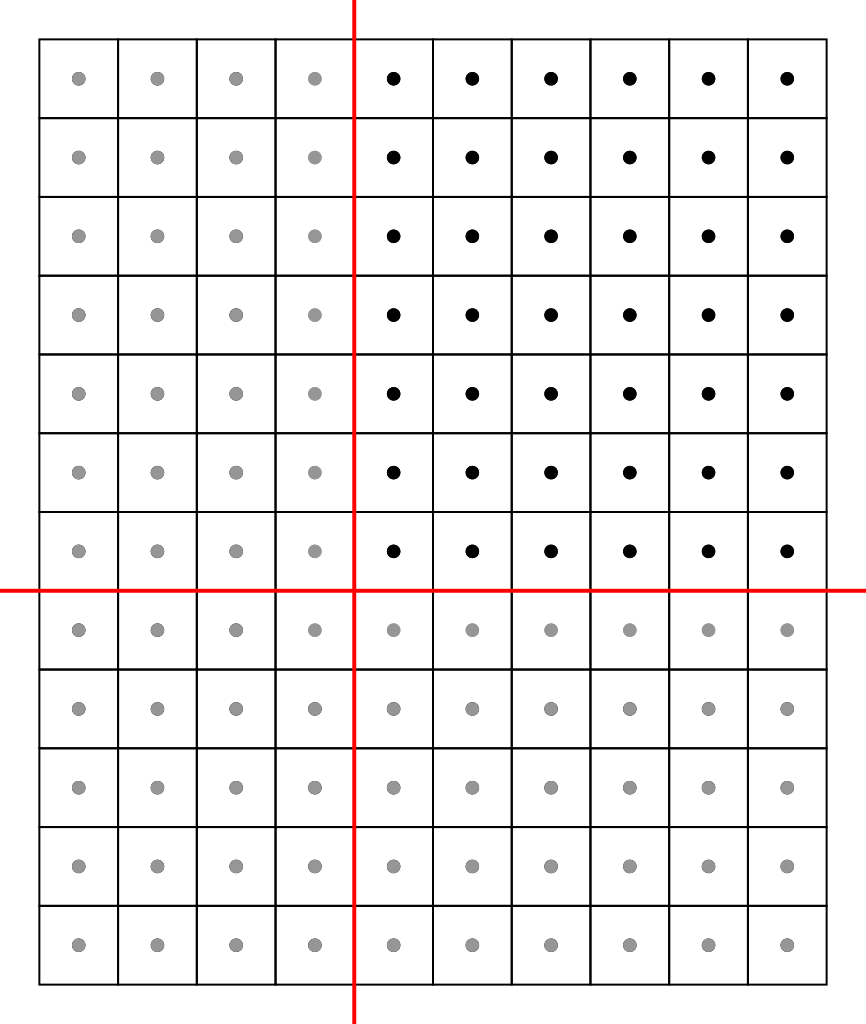
\includegraphics[width=0.75\linewidth]{grid-4}
    \end{center}
    \end{column}

    \begin{column}{0.5\linewidth}
    Sub-domain with ``ghosts''
      \begin{center}
      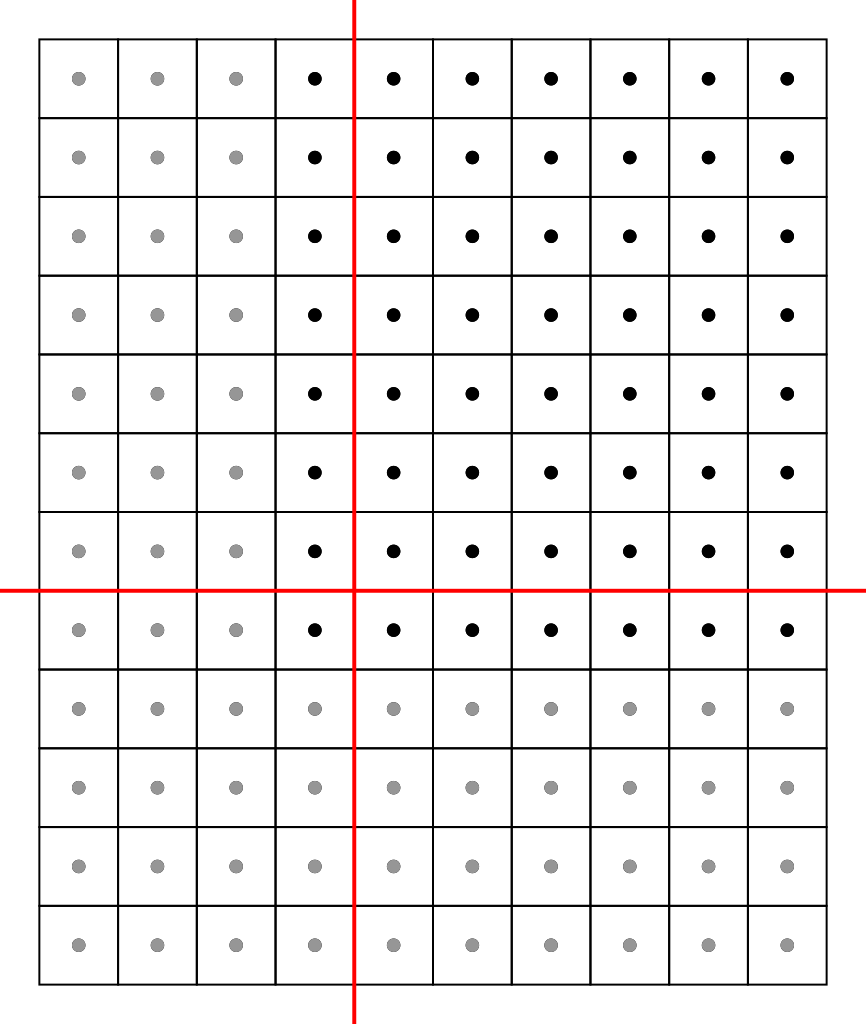
\includegraphics[width=0.75\linewidth]{grid-5}
    \end{center}
    \end{column}
  \end{columns}
\end{frame}

\begin{frame}[fragile]
  \frametitle{Working with 2D and 3D fields}

  Without ghosts:
\begin{lstlisting}
IceModelVec2S temperature(grid, "air_temp", WITHOUT_GHOSTS);

IceModelVec::AccessList access{&temperature};

for (Points p(grid); p; p.next()) {
  const int i = p.i(), j = p.j();

  temperature(i, j) = i + j;
}

temperature.update_ghosts();
\end{lstlisting}

  With ghosts:
\begin{lstlisting}
IceModelVec2S temperature(grid, "air_temp", WITH_GHOSTS, 1);

IceModelVec::AccessList access{&temperature};

for (PointsWithGhosts p(grid); p; p.next()) {
  const int i = p.i(), j = p.j();

  temperature(i, j) = i + j;
}
\end{lstlisting}
  
\end{frame}

\begin{frame}[fragile]
  \frametitle{Cell type mask}

  The cell type mask is often obtained from the \texttt{Geometry}
  object as \texttt{geometry.cell\_type}.

  \medskip
\begin{lstlisting}
  bool ocean(int i, int j) const;
  bool grounded(int i, int j) const;
  bool icy(int i, int j) const;
  bool grounded_ice(int i, int j) const;
  bool floating_ice(int i, int j) const;
  bool ice_free(int i, int j) const;
  bool ice_free_ocean(int i, int j) const;
  bool ice_free_land(int i, int j);
  //! Ice margin (ice-filled with at least one of four neighbors ice-free).
  bool ice_margin(int i, int j) const;
  //! Ice-free margin (at least one of four neighbors has ice).
  bool next_to_ice(int i, int j) const;
  bool next_to_floating_ice(int i, int j) const;
  bool next_to_grounded_ice(int i, int j) const;
  bool next_to_ice_free_land(int i, int j) const;
  bool next_to_ice_free_ocean(int i, int j) const;

\end{lstlisting}
\end{frame}

\newcommand{\var}[2]{ {#1}_{\text{#2}} }
\newcommand{\h}[1]{ \var{h}{#1} }
\newcommand{\T}[1]{ \var{T}{#1} }
\newcommand{\m}[1]{ \var{m}{#1} }

\begin{frame}
  \frametitle{Parameterizing surface temperature}
  \begin{align*}
    \diff{T}{h} &= (\T{max} - \T{min}) / (\h{max} - \h{min})\\
    \begin{split}T(x,y) &=
      \begin{cases}
        \T{min}, & h(x,y) \le \h{min}, \\
        \T{min} + \diff{T}{h} \, (h(x,y) - \h{min}), & \h{min} < h(x,y) < \h{max}, \\
        \T{max}, & \h{max} \le h(x,y).
      \end{cases}
    \end{split}\\
  \end{align*}
\end{frame}

 \begin{frame}
  \frametitle{Parameterizing surface mass balance}
  \begin{align*}
    \diff{\m{abl}}{h} &= -\m{min} / (\h{max} - \h{min})\\
    \diff{\m{acl}}{h} &= \m{max} / (\h{max} - \h{min})\\
    \begin{split}m(x,y) &=
      \begin{cases}
        \m{min}, & h(x,y) \le \h{min}, \\
        \diff{\m{abl}}{h} \, (h(x,y) - h_{\text{ELA}}), &  \h{min} < h(x,y) < \h{max}, \\
        \diff{\m{acl}}{h} \, (h(x,y) - h_{\text{ELA}}), & \h{min} < h(x,y) < \h{max}, \\
        \m{max}, & \h{max} \le h(x,y).
      \end{cases}\end{split}
  \end{align*}
\end{frame}

\begin{frame}[fragile]
  \frametitle{Elevation dependent T and SMB}
\begin{lstlisting}
class Elevation : public SurfaceModel {
public:
  Elevation(IceGrid::ConstPtr grid, std::shared_ptr<atmosphere::AtmosphereModel> input);
private:
  void init_impl(const Geometry &geometry);
  void update_impl(const Geometry &geometry, double t, double dt);

  MaxTimestep max_timestep_impl(double t) const;

  const IceModelVec2S& mass_flux_impl() const;
  const IceModelVec2S& temperature_impl() const;

  void compute_mass_flux(const IceModelVec2S &surface, IceModelVec2S &result) const;
  void compute_temperature(const IceModelVec2S &surface, IceModelVec2S &result) const;

  double m_T_min, m_T_max, m_z_T_min, m_z_T_max;
  double m_M_min, m_M_max, m_M_limit_min, m_M_limit_max, m_z_M_min, m_z_ELA, m_z_M_max;

  IceModelVec2S::Ptr m_mass_flux;
  IceModelVec2S::Ptr m_temperature;
};
\end{lstlisting}
\end{frame}

\begin{frame}[fragile]
  \frametitle{Elevation-dependent T and SMB: allocation}

\begin{lstlisting}
///// Elevation-dependent temperature and surface mass balance.
Elevation::Elevation(IceGrid::ConstPtr grid, std::shared_ptr<atmosphere::AtmosphereModel> input)
  : SurfaceModel(grid) {
  (void) input;

  m_temperature = allocate_temperature(grid);
  m_mass_flux   = allocate_mass_flux(grid);
}
\end{lstlisting}

\begin{lstlisting}
IceModelVec2S::Ptr SurfaceModel::allocate_temperature(IceGrid::ConstPtr grid) {

  IceModelVec2S::Ptr result(new IceModelVec2S(grid, "ice_surface_temp", WITHOUT_GHOSTS));

  result->set_attrs("climate_forcing",
                    "temperature of the ice at the ice surface but below firn processes",
                    "Kelvin", "");

  result->metadata().set_doubles("valid_range", {0.0, 323.15}); // [0C, 50C]

  return result;
}
\end{lstlisting}
\end{frame}

\begin{frame}[fragile,fragile]
  \frametitle{Elevation-dependent T and SMB: initialization}

\begin{lstlisting}
void Elevation::init_impl(const Geometry &geometry) {
  (void) geometry;

  bool limits_set = false;

  m_log->message(2,
                 "* Initializing the constant-in-time surface processes model Elevation...\n");

  units::Converter K(m_sys, "Celsius", "Kelvin");
  // options
  {
    // ice surface temperature
    {
      options::RealList IST("-ice_surface_temp", "ice surface temperature parameterization",
                            {-5.0, 0.0, 1325.0, 1350.0});

      if (IST->size() != 4) {
        throw RuntimeError(PISM_ERROR_LOCATION, "option -ice_surface_temp requires an argument"
                           " (comma-separated list of 4 numbers)");
      }
      m_T_min   = K(IST[0]);
      m_T_max   = K(IST[1]);
      m_z_T_min = IST[2];
      m_z_T_max = IST[3];
    }

  // more code processing command-line options (omitted)
  }
}

\end{lstlisting}
\end{frame}

\begin{frame}[fragile]
  \frametitle{Elevation-dependent T and SMB: update}
\begin{lstlisting}
MaxTimestep Elevation::max_timestep_impl(double t) const {
  (void) t;
  return MaxTimestep("surface 'elevation'");
}

void Elevation::update_impl(const Geometry &geometry, double t, double dt) {
  (void) t;
  (void) dt;

  compute_mass_flux(geometry.ice_surface_elevation, *m_mass_flux);
  compute_temperature(geometry.ice_surface_elevation, *m_temperature);
}
\end{lstlisting}
\end{frame}

\begin{frame}[fragile]
  \frametitle{Parameterizing mass flux}
\begin{lstlisting}
void Elevation::compute_mass_flux(const IceModelVec2S &surface,
                                  IceModelVec2S &result) const {
  double dabdz = -m_M_min/(m_z_ELA - m_z_M_min), dacdz = m_M_max/(m_z_M_max - m_z_ELA);

  IceModelVec::AccessList list{&result, &surface};

    for (Points p(*m_grid); p; p.next()) {
      const int i = p.i(), j = p.j();

      double z = surface(i, j);

      if (z < m_z_M_min) {
        result(i, j) = m_M_limit_min;
      }
      else if ((z >= m_z_M_min) and (z < m_z_ELA)) {
        result(i, j) = dabdz * (z - m_z_ELA);
      }
      else if ((z >= m_z_ELA) and (z <= m_z_M_max)) {
        result(i, j) = dacdz * (z - m_z_ELA);
      }
      else if (z > m_z_M_max) {
        result(i, j) = m_M_limit_max;
      }
      else {
        throw RuntimeError(PISM_ERROR_LOCATION,
                           "Elevation::compute_mass_flux: HOW DID I GET HERE?");
      }
    }

  // convert from m second-1 ice equivalent to kg m-2 s-1:
  result.scale(m_config->get_double("constants.ice.density"));
}
\end{lstlisting}
\end{frame}

\begin{frame}[fragile]
  \frametitle{Parameterizing surface temperature}
\begin{lstlisting}
void Elevation::compute_temperature(const IceModelVec2S &surface,
                                    IceModelVec2S &result) const {
  IceModelVec::AccessList list{&result, &surface};

  double dTdz = (m_T_max - m_T_min)/(m_z_T_max - m_z_T_min);

  ParallelSection loop(m_grid->com);
  try {
    for (Points p(*m_grid); p; p.next()) {
      const int i = p.i(), j = p.j();

      double z = surface(i, j);

      if (z <= m_z_T_min) {
        result(i, j) = m_T_min;
      }
      else if ((z > m_z_T_min) and (z < m_z_T_max)) {
        result(i, j) = m_T_min + dTdz * (z - m_z_T_min);
      }
      else if (z >= m_z_T_max) {
        result(i, j) = m_T_max;
      }
      else {
        throw RuntimeError(PISM_ERROR_LOCATION,
                           "Elevation::compute_temperature: HOW DID I GET HERE?");
      }
    }
  } catch (...) {
    loop.failed();
  }
  loop.check();
}

\end{lstlisting}
\end{frame}

\begin{frame}[fragile]
  \frametitle{Providing results to the rest of PISM}
\begin{lstlisting}

const IceModelVec2S &Elevation::mass_flux_impl() const {
  return *m_mass_flux;
}

const IceModelVec2S &Elevation::temperature_impl() const {
  return *m_temperature;
}

\end{lstlisting}
\end{frame}

\end{document}
% Local Variables:
% eval: (ws-butler-mode)
% eval: (flyspell-mode)
% End:
